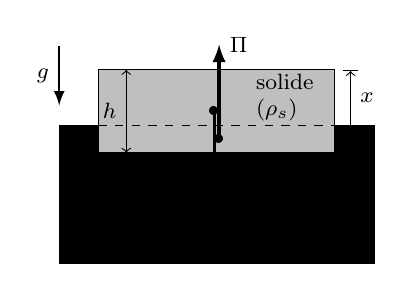
\begin{tikzpicture} [
	scale=1,
	font=\footnotesize,
	vecteur/.style={-latex,thick},
	force/.style={->,>=latex,draw=\JRLblue,very thick,nodes={\JRLblue}},
	liquide/.style={fill=\JRLblueC,very thin,draw=\JRLblueF},
    solide/.style={fill=lightgray},
	]
	% liquide
	\draw[liquide] (-2,0)--++(4,0)--++(0,-1.75)--++(-4,0)--cycle;
	\draw (-2,0)--++(4,0);
	\draw (0,-1.5) node{liquide ($\rho_\ell$)};
%	\draw (0,1.2) node[above]{air $(P_\text{atm})$};
	% solide
	\draw[solide,shift={(-1.5,-10pt)}](0,0)rectangle(3,30pt);
	\draw (1,22pt) node[below,text width=1cm]{solide ($\rho_\text{s}$)};
	\draw[dashed,thin] (-1.5,0)--++(3,0);	
	\draw[shift={(-1.5,-10pt)},<->](10pt,0)--++(0,30pt)node[midway,left]{$h$};
	\draw[->|](1.7,0)--++(0,20pt)node[midway,right]{$x$};
	% forces
	\draw[vecteur] (-2,1)--++(0,-0.75) node[pos=0.5,left]{$\vv{g}$};
	\draw[shift={(-1.53,-10pt)},force](1.5,15pt)node{•}--++(0,-1.2)node[right]{$\vv{P}$};
	\draw[shift={(-1.47,-10pt)},force](1.5,5pt)node{•}--++(0,1.2)node[right]{$\vv{\Pi}$};
%	\draw[help lines] (-2,-2) grid (2,2);
\end{tikzpicture}